\documentclass[11pt,largemargins]{homework}

\newcommand{\hwname}{Ornella Elena Grassi}
\newcommand{\hwemail}{s290310@studenti.polito.it}
\newcommand{\hwtype}{Homework}
\newcommand{\hwnum}{3}
\newcommand{\hwclass}{}
\newcommand{\hwlecture}{}
\newcommand{\hwsection}{}

% This is just used to generate filler content. You don't need it in an actual
% homework!
\usepackage{lipsum}
\usepackage{amssymb}
\usepackage[utf8]{inputenc}
\usepackage[T1]{fontenc}
\usepackage{lmodern}
\usepackage{amsfonts}
\usepackage{hyperref}
\usepackage{bbm}
\usepackage{amsmath}
\usepackage{mcode}
\usepackage{epstopdf}
\usepackage{subcaption}
\usepackage{amsmath}
\DeclareMathOperator*{\argmax}{argmax}
\DeclareMathOperator*{\argmin}{argmin}


\begin{document}
\maketitle
\begin{center}
Realizzato in collaborazione con Giulio Nenna (s245717), Andrea Sanna (s222975) e Alfredo Baione (s279328)
\end{center}
\section{}% --------------ESERCIZIO 1------------------------------
Si consideri il limite idrodinamico di diffusione epidemica SIR descritto dal sistema di equazioni differenziali
\begin{equation*}
\begin {cases} \dot{p}_{S}=-\alpha p_{S}p_{I}\\\dot{p}_{I}=p_{I}\left(\alpha p_{S}-1\right)\\\dot{p}_{R}=p_{I}\end{cases},
\end{equation*}
a partire dai nuclei di interazione descritti da
\begin{equation*}
\begin {cases} \Theta_{SI}\left(p\right)=\alpha p_{I}\\\Theta_{IR}\left(p\right)=1\end{cases}, \,\,\,\alpha>0.
\end{equation*}

 Sia $p\left(t\right)=\left(p_{S}\left(t\right),p_{I}\left(t\right),p_{R}\left(t\right)\right)$ la soluzione dell'ODE sopracitata, con la seguente condizione iniziale
 \begin{align*}
 p_{S}\left(0\right)=1-\epsilon, && p_{I}\left(0\right)=\epsilon,&&p_{R}\left(0\right)=0,
 \end{align*}
 dove $\epsilon \in ]0,1[$.
 \begin {alphaparts}
 \questionpart
 
  Per ricavare gli equilibri dell'ODE, risolviamo il sistema
  \begin{equation*}
\begin {cases} -\alpha p_{S}p_{I}=0\\p_{I}\left(\alpha p_{S}-1\right)=0\\p_{I}=0\\p_{S}+p_{I}+p_{R}=1\end{cases}\Leftrightarrow\begin {cases} p_{S}=1-p_{R}\\p_{I}=0\end{cases},
\end{equation*}
    da cui si ottengono i seguenti punti di equilibrio:
    \begin{align*}
    \left(\bar{p}_{S},\bar{p}_{I},\bar{p}_{R}\right)=\left(k,0,1-k\right), &&k\in[0,1].
    \end{align*}
  
 \questionpart
 Osserviamo che:
 \begin{equation*}
 \dot{p}_{S}=-\alpha p_{S}p_{I},
 \end{equation*}
  allora $\dot{p}_{S}\leq 0$ sempre e, dunque, $p_{S}$ è decrescente.\\
  Invece:
  \begin{equation*}
 \dot{p}_{R}=p_{I},
 \end{equation*}  
  quindi $\dot{p}_{R}\geq 0$ sempre e, pertanto, $p_{R}$ è crescente.
  
\questionpart
Dalla ODE possiamo ricavare che:
\begin{equation*}
\dot{p}_{I}\geq 0\Leftrightarrow \dot{p}_{S}\geq \frac{1}{\alpha}.
\end{equation*}  
Questo significa che, fintantoché $\dot{p}_{S}\geq \frac{1}{\alpha}$, $p_{i}$ sarà crescente; invece, nel caso in cui $\dot{p}_{S}\leq \frac{1}{\alpha}$, $p_{i}$ risulterà decrescente.
Avendo, però, dimostrato che $p_{S}$ è monotona decrescente, la soluzione dell'ODE, per $t \mapsto +\infty$, convergerà sempre ad un equilibrio della forma  $\left(\bar{p}_{S},\bar{p}_{I},\bar{p}_{R}\right)$.
Infatti, $p_{I}$ inizialmente o sarà crescente, per poi decrescere fino a $0$, oppure decrescerà soltanto fino a $0$. $\forall \epsilon$, dunque, l'equilibrio sarà raggiunto.

\questionpart
Riscriviamo l'equazione 
\begin{equation*}
\alpha x + \ln{\left(1-x\right)}
\end{equation*}
 così:
 
 
 \begin{align*}
 \ln{\left(\left(1-x\right)e^{\alpha x}\right)}. && \left(*\right)
 \end{align*}
  
 Dalla ODE possiamo ricavare l'espressione di $p_{R}$:
  \begin{equation*}
  p_{R}=\int p_{I}\,dt + c = \int -\frac{\dot{p}_{S}}{\alpha p_{S}} \,dt + c= -\frac{\ln{\left(p_{S}\right)}}{\alpha} + c.
  \end{equation*}
  Troviamo il valore di $c$:
  \begin{equation*}
  p_{R}\left(0\right)=-\frac{\ln{\left(p_{S}\left(0\right)\right)}}{\alpha} + c\Leftrightarrow \frac{\ln{\left(1-\epsilon\right)}}{\alpha} = c.
  \end{equation*}
  Pertanto:
  \begin{equation*}
  p_{R}=-\frac{\ln{\left(p_{S}\right)}}{\alpha} + \frac{\ln{\left(1-\epsilon\right)}}{\alpha}=\frac{1}{\alpha}\ln{\left(\frac{1-\epsilon}{p_{S}}\right)}.
  \end{equation*}
  Adesso, sapendo che il punto limite $\left(\bar{p}_{S},\bar{p}_{I},\bar{p}_{R}\right)$ è tale per cui
  \begin{align*}
  \bar{p}_{S}=1-\bar{p}_{R} \,\,\, \text{e} \,\,\, \bar{p}_{I}=0,
  \end{align*}
  sostituendo l'espressione di $\bar{p}_{R}$ nell'equazione $\left(*\right)$, otteniamo:
  \begin{equation*}
  \ln{\left(p_{S}\cdot e^{ln{\left(\frac{1-\epsilon}{p_{S}}\right)}}\right)}=\ln{\left(p_{S}\cdot\frac{1-\epsilon}{p_{S}}\right)}=\ln{\left(1-\epsilon\right)}.
  \end{equation*}
  
  \begin{figure}[htb]\centering
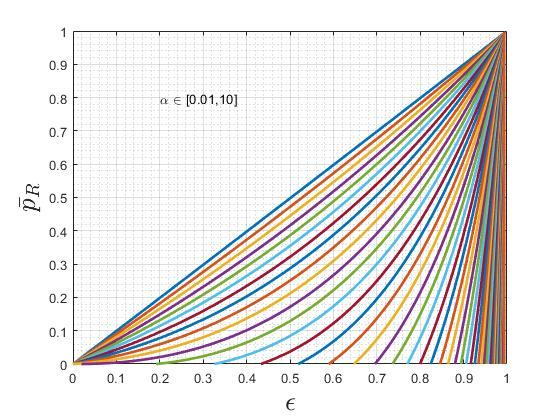
\includegraphics[scale=0.70]{plotex1_d.jpg}
  \end{figure}
  
  
  \newpage
 \questionpart
 Sia $\alpha < 1$.\\
 Dall'equazione dell'ODE si ricava che:
 \begin{equation*}
 \dot{p}_{I}=p_{I}\left(\alpha p_{S}-1\right)\leq p_{I}\left(\alpha-1\right),
\end{equation*}  
poiché se $\alpha<1$ e $p_{S}\leq 1$, risulta:
\begin{equation*}
\alpha p_{S}\leq \alpha.
\end{equation*}
\'E dunque possibile applicare il lemma di Gr\"onwall, dal momento che $\left(\alpha-1\right)$ e $p_{I}\left(t\right)$ sono funzioni continue a valori reali, definite su $[0,1]$, tali per cui $p_{I}\left(t\right)$ è derivabile in $]0,1[$.\\
Si avrà che:
\begin{equation*}
p_{I}\left(t\right)\leq p_{I}\left(0\right)e^{\left(\int_{0}^{t} \alpha-1 \,ds\right)}=\epsilon\cdot e^{\left(\alpha - 1\right)t}, \,\,\,\,\, t\geq 0.
\end{equation*}
Dal momento che
\begin{equation*}
\dot{p}_{R}\left(s\right)=p_{I}\leq \epsilon\cdot e^{\left(\alpha - 1\right)t}, \,\,\,\,\, t\geq 0,
\end{equation*}
integrando tra $0$ e $t$, otteniamo:
\begin{align*}
\int_{0}^{t} \dot{p}_{R} \,ds \leq \int_{0}^{t} \epsilon\cdot e^{\left(\alpha - 1\right)s} \,ds && \\
\Leftrightarrow p_{R}\left(t\right)\leq \frac{\epsilon\cdot e^{\left(\alpha - 1\right)t}}{\alpha-1} - \frac{\epsilon}{\alpha-1}= \frac{\epsilon}{1-\alpha}\left(1-e^{\left(\alpha-1\right)t}\right), \,\,\,\,\, t\geq 0.
\end{align*}
Da tale risultato si ricava che:
\begin{equation*}
\bar{p}_{R}=\lim\limits_{t \rightarrow +\infty}p_{R}\left(t\right)\leq \lim\limits_{t \rightarrow +\infty}\frac{\epsilon}{1-\alpha}\left(1-e^{\left(\alpha-1\right)t}\right)=\frac{\epsilon}{1-\alpha}\left(1-0\right)=\epsilon\left(1-\alpha\right)^{-1}.
\end{equation*}

\questionpart
Sia $\alpha>1$ e $\left(1-\epsilon\right)\alpha>1$.\\
Dunque, siamo nel caso in cui $p_{S}$ può assumere, ad un certo istante $\bar{t}$, il valore $\frac{1}{\alpha}$, poiché $\frac{1}{\alpha}<1$, $p_{S}$ è decrescente e $p_{S}\left(0\right)>\frac{1}{\alpha}$ (per ipotesi).\\
Siccome $\dot{p}_{I}>0$ fintantoché $p_{S} >\frac{1}{\alpha}$ e $\dot{p}_{I}<0$ quando $p_{S}<\frac{1}{\alpha}$, questo significa proprio che $\bar{t}$ è un punto di massimo assoluto per $p_{I}$.\\
Ne consegue che $p_{I}$ sarà crescente in $[0,\bar{t}]$ e decrescente in $[\bar{t},+\infty[$.

\questionpart
Sia $\alpha>1$.\\
Per capire se, in tal caso, $\bar{p}_{R}$ ammette un limite dal basso, è possibile studiare i punti critici dell'equazione di cui $\bar{p}_{R}$ è soluzione, nell'intervallo $[0,1[$.\\
Osserviamo che, per quanto visto prima, $\bar{p}_{R}$ è sempre limitato dall'alto da
\begin{equation*}
\lim\limits_{t \rightarrow +\infty}\frac{\epsilon}{1-\alpha}\left(1-e^{\left(\alpha-1\right)t}\right),
\end{equation*}
soltanto che, questa volta, siccome $\alpha>1$, tale limite va a $+\infty$.\\
Sia
\begin{equation*}
f\left(x\right)=\alpha x +  \ln{\left(1-x\right)}.
\end{equation*}
Si avrà:
\begin{equation*}
f\left(x\right)'=\alpha - \frac{1}{1-x}\geq 0\Leftrightarrow x\leq 1-\frac{1}{\alpha}
\end{equation*}
e, pertanto, $f\left(1-\frac{1}{\alpha}\right)$ risulta essere un massimo per $f\left(x\right)$.\\Inoltre, dato che $f\left(0\right)>0$ e la funzione è crescente nell'intervallo $[0,1-\frac{1}{\alpha}]$, essa si annullerà necessariamente in corrispondenza di $\bar{p}_{R}$ tale che
\begin{equation*}
1-\frac{1}{\alpha}\geq \bar{p}_{R}.
\end{equation*}  
\end{alphaparts}
% Sometimes questions get separated from their bodies. Use a \newpage to force
% them to wrap to the next page.
% Use \renewcommand{\questiontype}{<text>} to change what word is displayed
% before numbered questions
%\renewcommand{\questiontype}{Task}

\section{} %------ ESERCIZIO 2 ---------------------------------------
Sia  \(\mathcal{G}=(\mathcal{V}, \varepsilon, W)\) un grafo di ordine \(n = | \mathcal{V}| \geq 2\) privo di self loop tale che ogni nodo abbia grado uscente \(\omega_i > 0\). Si considera un gioco tra i giocatori \(\mathcal{V}\), ciascuno con spazio delle azioni \(\mathcal{A} = \mathbb{R}\) e funzioni di utilità
\begin{gather*}
  u_i(x)=- \frac{x_i^2}{2}+ c_i x_i + \beta \sum\limits_{j \neq i} W_{ij}x_j x_i 
\end{gather*} 
con \(i \in \mathcal{V} \), \(\beta \geq 0\) e \(c \in \mathbb{R}^{\mathcal{V}}\).
\begin{alphaparts}
  \questionpart %--------------------------------------------------
  Dal momento che  il grafo non presenta \textit{self-loop} allora \(W\) ha elementi tutti nulli sulla diagonale. Ci si può pertanto ricondurre alla scrittura matriciale:
  \begin{gather*}
    u_i(x)=- \frac{x_i^2}{2}+ c_i x_i + \beta ( Wx )_i x_i
  \end{gather*}
  Per lo stesso motivo il termine \(\beta(Wx)_i\) non dipende da \(x_i\) pertanto:
  \begin{gather}
    \frac{\delta u_i ( x )}{\delta x_i} = -x_i + c_i + \beta (Wx)_i
  \end{gather} \label{eq:1}
  Ponendo quindi quest'ultima quantità pari a 0, poiché \(u_i(x)\) è una funzione quadratica concava, si ottiene:
  \begin{gather*}
    BR_i(x^{-i}) = c_i + \beta  \sum \limits_{j \neq i}^{} W_{ij}x_j 
  \end{gather*}

  \questionpart %-----------------------------------------------------
  Gli equilibri di Nash si realizzano nelle configurazioni \(x^*\) in cui ogni giocatore assume la sua \textit{best-response}, pertanto dalla \ref{eq:1}:
  \begin{gather*}
    x^* = c + \beta W x^* 
  \end{gather*}
  Quindi gli equilibri di Nash saranno nella forma
  \begin{gather*}
    x^* = (I-\beta W)^{-1}c
  \end{gather*}
  L'esistenza e unicità di \(x^*\) dipende quindi solamente dall'invertibilità di \((I-\beta W)\). Siano pertanto \(\lambda_i\) gli autovalori di \(W\), allora \(\psi_i = (1 - \beta \lambda_i)\) sono gli autovalori di \((I-\beta W)\). Affinché questa sia quindi invertibile deve valere \(\forall i \in \{1, \dots n\}\) 
  \begin{gather*}
    \psi_i \neq 0 \Rightarrow \beta \lambda_i \neq 1
  \end{gather*}
  L'equilibrio di Nash \(x^*\) esiste ed è unico se e solo se vale quindi:
  \begin{align*}
    \beta \neq \frac{1}{\lambda_i} && \forall \lambda_i \in \sigma(W)
  \end{align*} 
  Si pone ora \begin{align} \label{eq:2}
    \beta \omega_i < 1 && \forall i \in \mathcal{V}
  \end{align} ossia le righe di \(\beta W\) sommano ad una quantità strettamente minore di 1, quindi \(\beta W\) è \textit{substocastica}. Questo vuol dire che per il suo raggio spettrale vale \(\rho(W)<1\) e può quindi essere applicato il \textit{Criterio di Neumann} che non solo ci assicura l'esistenza di \((I-\beta W)^{-1}\) ma ci fornisce anche il seguente risultato:
  \begin{gather*}
    (I-\beta W)^{-1} =  \sum \limits_{k=0}^{\infty} \beta^k W^k
  \end{gather*}

  \questionpart %-----------------------------------------------------
  Come visto nel punto precedente, se \((I-\beta W)\) è invertibile allora esiste ed è unico l'equilibrio di Nash \(x^*\). In particolare se si pone \((I-\beta W)^{-1} = M \) allora vale:
  \begin{gather*}
    x^* = Mc
  \end{gather*}
  pertanto il vettore \(x^*\) dipende linearmente dal vettore \(c\).\\
  Se inoltre vale \ref{eq:2} allora:
  \begin{gather*}
    M= \sum \limits_{k=0}^{\infty} \beta^k W^k
  \end{gather*}
  e poiché per costruzione \(\beta > 0\) e \(W_{ij}\geq 0 \) \(\forall i,j \in \mathcal{V}\) allora necessariamente
  \begin{align*}
    M_{ij} \geq 0 && \forall i,j \in \mathcal{V} .
  \end{align*}


  \questionpart %-----------------------------------------------------
  Il vettore di centralità di Katz si può esprimere nella forma seguente: 
  \begin{gather*}
    z = \left(I - \left(\frac{1-\beta_k}{\lambda_W}\right)W'\right)^{-1}\beta_k \mu
  \end{gather*}
  Poiché \(\beta_k\) e \(\mu\) sono rispettivamente il fattore di attenuazione della rete e il vettore di \textit{centralità intrinseca}, entrambi scelti arbitrariamente, è possibile porre i seguenti valori:
  \begin{gather*}
    \beta_k = 1-\beta \lambda_W \\
    \mu = \frac{1}{\beta_k}\mathbbm{1}.
  \end{gather*}
  Si ottiene quindi:
  \begin{gather*}
    z = (I- \beta W')^{-1} \mathbbm{1}
  \end{gather*}
  che in forma scalare equivale a:
  \begin{align}
    z_i =  \sum \limits_{j=1}^{n} (I- \beta W')_{ij}^{-1} && \forall i\in \mathbb{V}.
  \end{align}
  Si sviluppa ora il termine \(y =  \sum \limits_{j=1}^{n} x_j^*\) applicando il criterio di Neumann alla matrice \(M\) e scambiando indici e sommatorie al fine di mostrare che \(y =\langle c, z\rangle \):
  \begin{gather*}
    y =  \sum \limits_{j=1}^{n} x_j^* =  \sum \limits_{j=1}^{n}  \sum \limits_{i=1}^{n} (I-\beta W)^{-1}_{ji} c_i = \\
    =  \sum \limits_{j=1}^{n}  \sum \limits_{i=1}^{n}  \sum \limits_{k=0}^{\infty} \beta^k W_{ji}^k c_i =  \sum \limits_{i=1}^{n}  \sum \limits_{j=1}^{n}  \sum \limits_{k=0}^{\infty} \beta^k W_{ji}^k c_i = \\
     \sum \limits_{i=1}^{n} c_i  \sum \limits_{j=1}^{n}  \sum \limits_{k=0}^{\infty} \beta ^ k W_{ij}^{'k} =  \sum \limits_{i=1}^{n} c_i   \sum \limits_{j=1}^{n} (I-\beta W ')^{-1}_{ij} \\
     =  \sum \limits_{i=1}^{n}c_i z_i = \langle c, z \rangle 
  \end{gather*}

  \questionpart %-------------------------------------------------------
  Essendo \(c_i\) variabili aleatorie indipendenti \(Cov(c_i, c_j)=0\), pertanto vale:
  \begin{gather*}
    Var(y)=Var\left( \sum \limits_{i=1}^{n} z_i c_i\right) =  \sum \limits_{i=1}^{n} z_i^2 \sigma_i^2
  \end{gather*}

  \questionpart %--------------------------------------------------------
  Eliminando un qualsiasi giocatore \(i\) dal gioco, le proprietà della matrice \(W^{(-i)}\) sono le stesse della matrice \(W\). Pertanto se continua a valere \ref{eq:2} allora la matrice \((I-\beta W^{(-1)})\) è ancora substocastica. In particolare se \(c = \mathbbm{1}\) allora, grazie al criterio di Neuman esiste ed è unico un vettore \(x^{*(-i)}\) tale che 
  \begin{gather*}
    x^{*(-i)}  = (I-\beta W^{(-i)})^{-1} \mathbbm{1}
  \end{gather*}

  \questionpart 
  Per ogni \(k \neq i \neq j\) vale:
  \begin{gather*}
    M_{ij}M_{ik} = M_{ii}(M_{ij}-M_{ij}^{(-i)}).
  \end{gather*}
  \questionpart%---------------------------------------------------------
  Sia \(\mathcal{V}^{(-i)} := \mathcal{V}\backslash \{i\}\). Sappiamo che \(M\) e \(M^{(-i)}\) sono matrici con elementi non negativi, quindi:
  \begin{gather*}
    y = \sum \limits_{j \in \mathcal{V}} x_j^* = \sum \limits_{j \in \mathcal{V}} (M\mathbbm{1})_j = \sum \limits_{j \in \mathcal{ V}} \sum \limits_{k \in \mathcal{ V}} M_{jk} > 0   
    \\  y^{(-i)} = \sum \limits_{j \neq i} x_j^{*(-i)} = \sum \limits_{j \in \mathcal{V}^{(-i)}} (M\mathbbm{1})_j = \sum \limits_{j \in \mathcal{ V}^{(-i)}} \sum \limits_{k \in \mathcal{ V}^{(-i)}} M^{(-i)}_{jk} > 0   
  \end{gather*}
  Inoltre vale:
  \begin{gather*}
    z_i = \sum \limits_{j \in \mathcal{V}} M_{ij} \Rightarrow \frac{z_i^2}{M_{ii}} =\frac{1}{M_{ii}} \sum \limits_{j \in \mathcal{V}} \sum \limits_{k \in \mathcal{V}} M_{ij}M_{ik} 
  \end{gather*}
  Utilizzando il punto (g) e considerando \(M_{jk}^{(-i)}=0\) se \(j = i\) oppure \(k=i\) , vale:
  \begin{gather*}
    \frac{1}{M_{ii}} \sum \limits_{j \in \mathcal{V}} \sum \limits_{k \in \mathcal{V}} M_{ij}M_{ik} = \frac{1}{M_{ii}}\sum \limits_{j \in \mathcal{V}} \sum \limits_{k \in \mathcal{V}} M_{ii}(M_{jk}-M_{jk}^{(-i)}) = \\
     \sum \limits_{j \in \mathcal{V}} \sum \limits_{k \in \mathcal{V}} M_{jk} - \sum \limits_{j \in \mathcal{V}} \sum \limits_{k \in \mathcal{V}} M_{jk}^{(-i)} = \sum \limits_{j \in \mathcal{V}} \sum \limits_{k \in \mathcal{V}} M_{jk} - \sum \limits_{j \in \mathcal{V}^{(-i)}} \sum \limits_{k \in \mathcal{V}^{(-i)}} M_{jk}^{(-i)} =
     \\ y - y^{(-i)}
  \end{gather*}
  Utilizzando tutti questi risultati si ottiene quindi
  \begin{gather*}
    \frac{z_i^2}{M_{ii}} =  y - y^{(-i)}  \Rightarrow \argmax \limits_{i \in \mathcal{V}} y - y^{(-i)} = \argmax \limits_{i \in \mathcal{V}}\frac{z_i^2}{M_{ii}}
  \end{gather*}
  %\begin{gather*}
    %\argmax \limits_{i \in \mathcal{V}} y - y^{(-i)} = \argmin \limits_{i \in \mathcal{V}} y^{(-i)} = 
   % \argmin \limits_{i \in \mathcal{V}}\left( \sum \limits_{j \in \mathcal{ V}^{(-i)}} \sum \limits_{k \in \mathcal{ V}^{(-i)}} M^{(-i)}_{jk}  \right).
 % \end{gather*}
  %Utilizzando il punto (g) si ottiene:
  %\begin{gather*}
   % \argmin \limits_{i \in \mathcal{V}}\left( \sum \limits_{j \in \mathcal{ V}^{(-i)}} \sum \limits_{k \in \mathcal{ V}^{(-i)}} M^{(-i)}_{jk}  \right) = \argmin \limits_{i \in \mathcal{V}}\sum \limits_{j \in \mathcal{ V}^{(-i)}} \sum \limits_{k \in \mathcal{ V}^{(-i)}} \left(\frac{M_{ii}M_{jk}-M_{ij}M_{ik}}{M_{ii}}\right) = \\
   % \argmin \limits_{i \in \mathcal{V}} \left(\sum \limits_{j \in \mathcal{ V}^{(-i)}} \sum \limits_{k \in \mathcal{ V}^{(-i)}} M_{jk}- \sum \limits_{j \in \mathcal{ V}^{(-i)}} \sum \limits_{k \in \mathcal{ V}^{(-i)}} \frac{M_{ij}M_{ik}}{M_{ii}} \right) = \\
   % \argmax \limits_{i \in \mathcal{V}} \left(\sum \limits_{j \in \mathcal{ V}^{(-i)}} \sum \limits_{k \in \mathcal{ V}^{(-i)}} \frac{M_{ij}M_{ik}}{M_{ii}} \right).
  %\end{gather*}
  

  \questionpart
  \begin{figure}[htb]\centering
    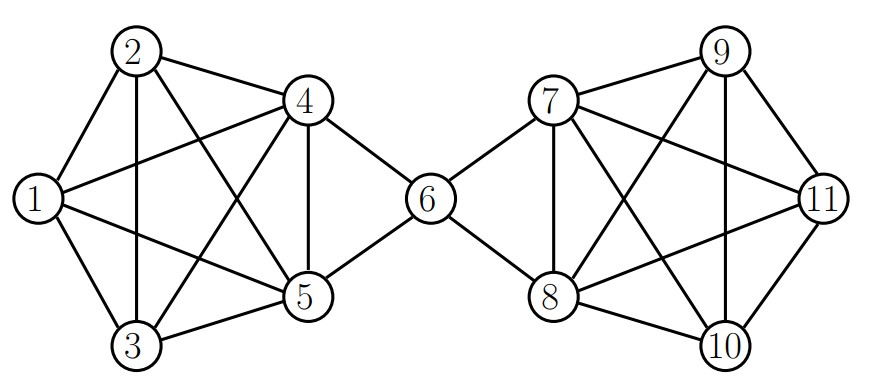
\includegraphics[scale=0.40]{Grafo.jpg}
      \end{figure}
  Siano
  \begin{gather*}
    \pi_a = \{1 , 2, 3, 9, 10, 11\}\\
    \pi_b = \{4, 5, 7, 8\}\\
    \pi_c = \{6\}
  \end{gather*}
  i gruppi di simmetria del grafo in figura. Supponiamo che
  \begin{align*}
    z_i = z_a && \forall i \in \pi_a \\
    z_i = z_b && \forall i \in \pi_b \\
    z_6 = z_c.\\
  \end{align*}
  Vale inoltre il seguente:
  \begin{gather*}
    z = M\mathbbm{1} = (I-\beta W')^{-1}\mathbbm{1} \Rightarrow (I-\beta W')z = \mathbbm{1} \\
    \Rightarrow z = \mathbbm{1} + \beta W' z
  \end{gather*}
  Si ottiene quindi il seguente sistema:
  \begin{gather*}
    \begin{cases}
      z_a = 1 + \beta (2z_a + 2z_b)\\
      z_b = 1+ \beta (3z_a + z_b + z_c)\\
      z_c = 1+ 4\beta z_b
    \end{cases}
  \end{gather*}
  da cui si ottengono le seguenti soluzioni:
  \begin{align*}
    \begin{cases}
      z_{1a} = 1.72 \\
      z_{1b}= 1.87 \\
      z_{1c} = 1.75
    \end{cases} && \begin{cases}
      z_{2a} = 7.77 \\
      z_{2b} = 9.16 \\
      z_{2c} = 8.33
    \end{cases}
  \end{align*}
  Dove \(z_1\) e \(z_2\) rappresentano i vettori di centralità di Katz calcolati rispettivamente nel caso in cui \(\beta = 0.1\) e \(\beta = 0.2\). Analogamente siano \(M^1 = (I-0.1W)^{-1}\) e \(M^2 = (I-0.2W)^{-1}\), si ottengono i seguenti risultati:
  \begin{align*}
    \begin{cases}
      M^1_a = 1.06\\
      M^1_b = 1.07\\
      M^1_c = 1.05
    \end{cases} &&
    \begin{cases}
      M^2_a = 1.85\\
      M^2_b = 2.08\\
      M^2_c = 1.66
    \end{cases}
  \end{align*}
  Dove \(M_{ii} = M_k \) \(\forall i \in \pi_k\) , \(k=\{a,b,c\}\).\\
  In entrambi i casi i nodi che massimizzano il rapporto \(z_i^2 / M_{ii}\) sono quelli del gruppo \(b\), infatti:
  \begin{align*}
    \frac{z_{1b}^2}{M_b^1}=3.281 && \frac{z_{2b}^2}{M_b^2}=40.33 
  \end{align*}


\end{alphaparts}
\end{document}
